% Two overlapping charts on S^1 and the transition map phi_{12}.
% Source: book/tex/diffgeo/manifolds.tex (§ Transition maps).
\documentclass[border=2mm]{standalone}
\usepackage{tikz}\usetikzlibrary{arrows.meta}\usepackage{amssymb}
\begin{document}
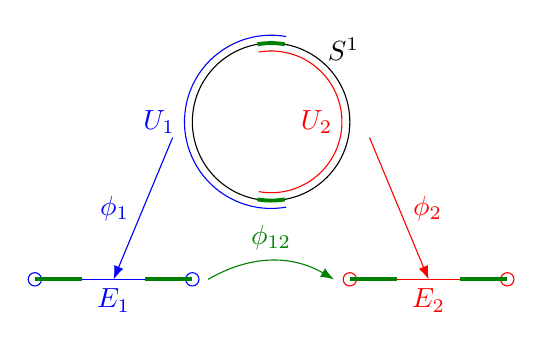
\begin{tikzpicture}
  \draw[black] (0,0) circle (1); \node at (45:1.3) {$S^1$};
  \draw[green!50!black,line width=1.4pt] (80:1) arc (80:100:1);
  \draw[green!50!black,line width=1.4pt] (-100:1) arc (-100:-80:1);
  \draw[red] (-100:0.9) arc (-100:100:0.9); \node[red,left] at (0:0.9) {$U_2$};
  \draw[blue] (80:1.1) arc (80:280:1.1); \node[blue,left] at (180:1.1) {$U_1$};
  \draw[blue] (-3,-2)--(-1,-2); \draw[blue,fill=white](-3,-2)circle(2.4pt);\draw[blue,fill=white](-1,-2)circle(2.4pt);
  \node[blue,below] at (-2,-2) {$E_1$};
  \draw[blue,-{Latex}] (-1.25,-0.2)--(-2,-2); \node[blue,left] at (-1.68,-1.1){$\phi_1$};
  \draw[red] (1,-2)--(3,-2); \draw[red,fill=white](1,-2)circle(2.4pt);\draw[red,fill=white](3,-2)circle(2.4pt);
  \node[red,below] at (2,-2){$E_2$};
  \draw[red,-{Latex}] (1.25,-0.2)--(2,-2); \node[red,right] at (1.68,-1.1){$\phi_2$};
  \draw[green!50!black,line width=1.4pt] (-3,-2)--(-2.4,-2);
  \draw[green!50!black,line width=1.4pt] (-1,-2)--(-1.6,-2);
  \draw[green!50!black,line width=1.4pt] (1,-2)--(1.6,-2);
  \draw[green!50!black,line width=1.4pt] (3,-2)--(2.4,-2);
  \draw[green!50!black,-{Latex}] (-0.8,-2) to[bend left=30] (0.8,-2);
  \node[green!50!black,above] at (0,-1.75) {$\phi_{12}$};
\end{tikzpicture}
\end{document}
